% \section{Related Work}
% \label{sec:related}

% % \subsection{FAST: Full-stack Accelerator Search Technique}
% % \begin{figure}[ht!]
% %     \centering
% %     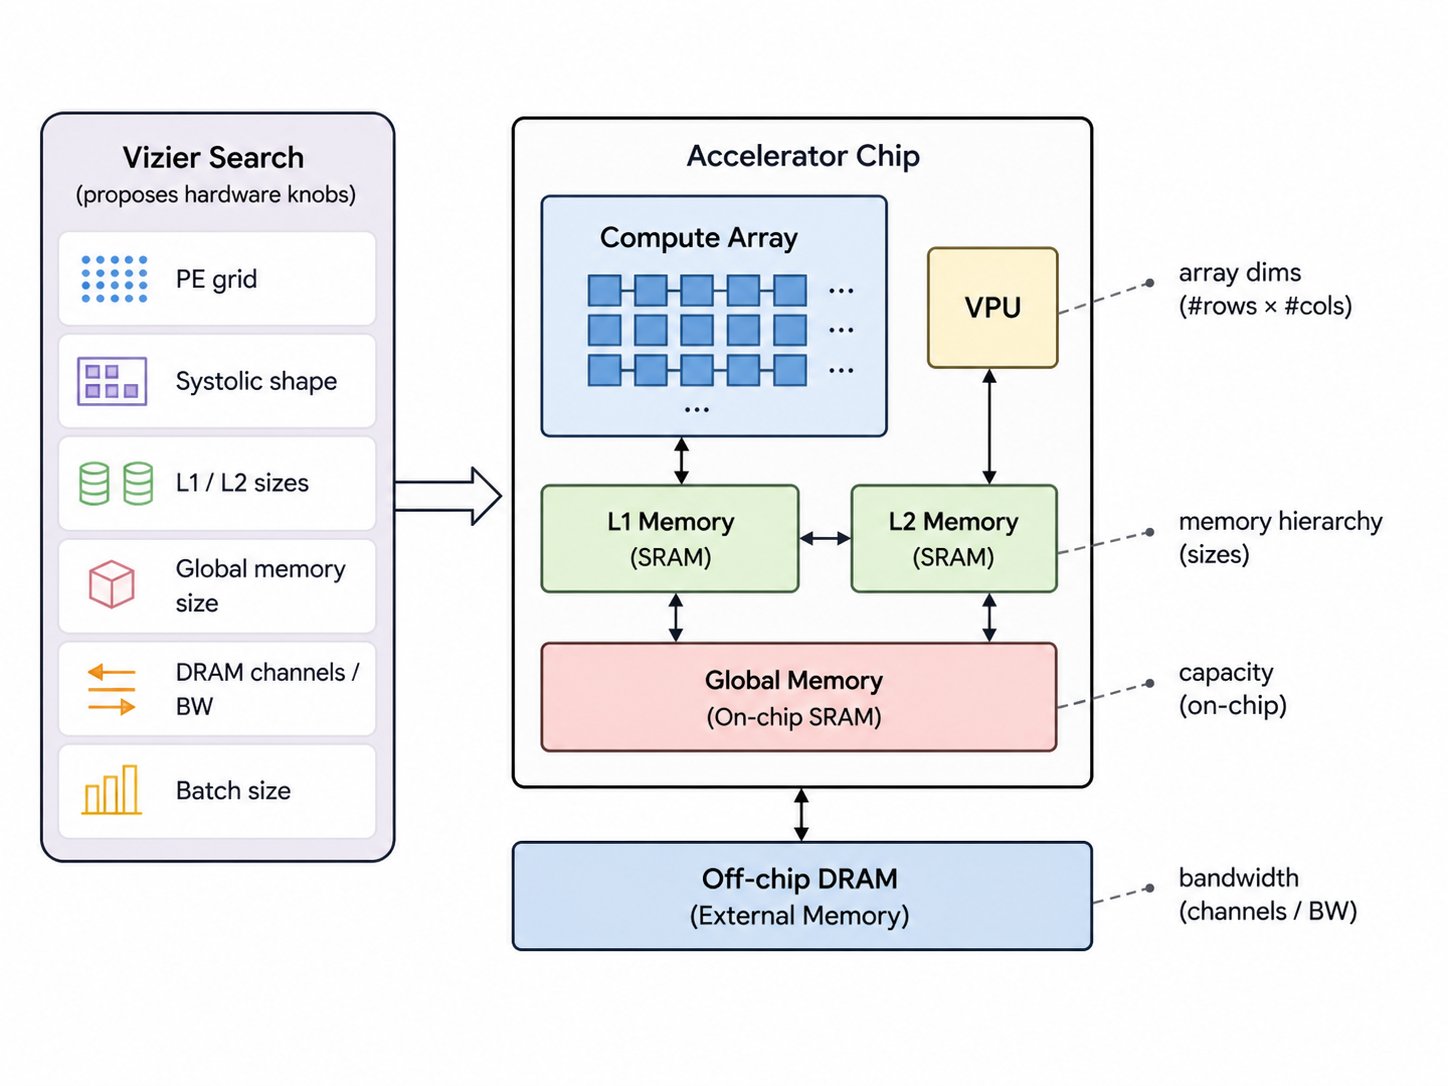
\includegraphics[width=0.5\linewidth]{figs/hardware_layout.png}
% %     \caption{The accelerator datapath template. Processing elements (PEs) are arranged in a grid connected by a mesh network. Each PE contains a systolic array for matrix operations, a vector processing unit (VPU) for non-MAC operations, and private or shared L1/L2 memory. A Global Memory serves as the on-chip scratchpad shared across all PEs. FAST-CORGI jointly optimizes how operations are tiled across this memory hierarchy and which tensors are pinned in Global Memory, replacing the sequential tiling$\rightarrow$fusion pipeline of FAST.}
% %     \label{fig:pipeline}
% % \end{figure}
% % FAST designs inference accelerators by jointly searching over hardware datapaths, software schedules, and compiler passes.
% % It targets a general ML accelerator template (Figure~\ref{fig:pipeline}) consisting of a grid of processing elements (PEs), each containing a systolic array for matrix operations and a vector processing unit (VPU) for non-MAC operations such as softmax and layer normalization.
% % The memory hierarchy includes per-PE L1 scratchpads, optional L2 buffers, a shared Global Memory, and off-chip DRAM.
% % The full hardware configuration is defined by 16 hyperparameters---PE grid dimensions, systolic array sizes, buffer capacities, DRAM channels, and batch size---spanning a datapath search space of $\mathcal O(10^{13})$ \citep[Table~3]{zhang_fast}.

% % FAST operates as a three-stage sequential pipeline within each trial of Google's Vizier:
% % (1)~Vizier proposes a hardware configuration;
% % (2)~Timeloop~ finds the best tiling and mapping for each operation independently, given the fixed hardware, producing per-operation execution time estimates;
% % (3)~an integer linear program (ILP) decides which tensors to pin in the Global Memory to reduce DRAM traffic, given the fixed per-operation schedules.
% % The predicted Perf/TDP is returned to Vizier, which proposes the next configuration.
% % This cycle repeats for ${\sim}5000$ trials.

% % FAST-generated accelerators achieve $3.7\times$ average Perf/TDP improvement over TPU-v3 across vision and NLP workloads~\citep[Section~6.2]{zhang_fast}.
% % However, the sequential decomposition means each stage commits to decisions that downstream stages cannot revise---Timeloop optimizes each operation's tiling without considering how its working-set size affects fusion feasibility, and the fusion ILP cannot request alternative tilings that might enable better global solutions.
% % Our work addresses this limitation by replacing stages~(2) and~(3) with a joint LP formulation.

% % \subsection{Related work.}
% \paragraph{Accelerator design space.} Hardware/Software (HW/SW) design exploration has been widely studied through tools
% that optimize datapath configurations and operation mappings, including
% Eyeriss~\citep{chen2019eyerissv2flexibleaccelerator},
% Timeloop~\citep{timeloop},
% MAESTRO~\citep{kwon2020understandingreuseperformancehardware},
% Interstellar~\citep{yang_interstellar},
% CoSA~\citep{huang2021cosaschedulingconstrainedoptimization},
% and ZigZag~\citep{mei2021zigzag}.
% FAST advanced the field by presenting a tractable way to comprehensively search over datapath,
% schedule, and compiler passes. This demonstrated the potential of co-design to achieve speedups for targeted neural network workloads that can achieve $3.7\times$ Perf/TDP improvement over a standard TPU-v3 baseline.
% However, within single trial involves a sequential flow through 3 components(Vizier for hardware candidate proposal, Timeloop for tiling, and and ILP solver for fusion), for a total of 5000 trials which may take days.
% This imitates the standard human engineering sequential pipeline of designing domain optimized deep learning accelerators---each stage consumes the previous
% stage's output as fixed. Tiling and fusion have mature but separate
% literatures: tiling builds on loop optimization techniques from
% Halide~\citep{ragan2013halide} and Ansor~\citep{zheng2023ansorgeneratinghighperformancetensor},
% while fusion extends compiler passes in XLA and training-time
% rematerialization~\citep{chen2016trainingdeepnetssublinear,
% jain2020checkmatebreakingmemorywall}. Recent work has begun to address joint tiling and fusion optimization:
% TileFlow \citep{zheng2023tileflow} explores fusion dataflows via tree-based
% analysis, and FADiff \citep{jia2025fadifffusionawaredifferentiableoptimization} formulates a differentiable
% joint mapping-fusion objective. Our formulation differs in targeting hardware-software
% co-design with a large-scale LP that provides valid lower bounds via exact
% bilinear linearization, and additionally handles rematerialization
% and dynamic memory scheduling for datacenter-scale accelerators.

% \paragraph{Optimization Techniques.} Our joint LP reformulation is enabled by McCormick
% envelopes~\citep{mccormick1976computability}, which exactly linearize
% the bilinear tiling$\times$placement interaction, and by scalable first-order
% LP solvers descended from PDLP~\citep{applegate2022practicallargescalelinearprogramming}.
% For the outer hardware search loop, we draw on recent work using LLMs as
% informed mutation operators---FunSearch~\citep{romera2024mathematical},
% AlphaEvolve~\citep{novikov2025alphaevolvecodingagentscientific}, and
% EvoPrompting~\citep{chen2023evopromptinglanguagemodelscodelevel}---to
% propose hardware configurations guided by workload bottleneck analysis and prior trial results.
% A full discussion of related work appears in Appendix~\ref{related_work_appendix}.
% % \subsection{Related Work}
% % \paragraph{Accelerator design space exploration.}
% % Hardware ML accelerators are characterized by their datapath (compute units, memory hierarchy, interconnect) and software schedule (how operations map onto hardware).
% % A substantial body of work explores design spaces of accelerator families by mutating datapath hyperparameters and operation mappings.
% % % Eyeriss
% % \citep{chen2019eyerissv2flexibleaccelerator} introduced Eyeriss, a spatial architecture with a row-stationary dataflow for energy-efficient CNNs.
% % % Timeloop
% % \citep{timeloop} proposed Timeloop, a systematic infrastructure for evaluating DNN accelerator schedules and datapaths.
% % % MAESTRO
% % \citep{kwon2020understandingreuseperformancehardware} developed MAESTRO, a data-centric framework for understanding DNN mapping performance.
% % % Interstellar
% % \citep{yang_interstellar} used Halide's scheduling language to analyze DNN accelerators in Interstellar.
% % % dMazeRunner
% % \citep{dave2019dmazerunner} optimized convolution mappings on dataflow accelerators with dMazeRunner. 
% % % MAGNet
% % \citep{venkatesan2019magnet} proposed MAGNet, a modular accelerator generator, reporting up to 1.75$\times$ Perf/W improvement.
% % % Apollo
% % \citep{yazdanbakhsh2021apollotransferablearchitectureexploration} explored transferable architecture exploration via Apollo.
% % % ConfuciuX
% % \citep{kao2020confuciuxautonomoushardwareresource} applied reinforcement learning to hardware resource assignment.
% % % CoSA
% % Huang \etal~formulated accelerator mapping as a constrained optimization problem in CoSA \citep{huang2021cosaschedulingconstrainedoptimization}.
% % FAST extended these approaches by jointly optimizing datapath, schedule, and compiler passes including operation fusion, achieving $3.7\times$ average Perf/TDP improvement over TPU-v3 across vision and language workloads.
% % Our work preserves FAST's outer hardware search loop but replaces the sequential inner optimization with a joint linear program.


% % \paragraph{Operation fusion and memory optimization.}
% % Operation fusion reduces DRAM traffic by keeping intermediate tensors on-chip.
% % Production compilers such as XLA fuse simple patterns, but each fusion region contains at most one matrix operation.
% % FAST introduced an ILP-based fusion technique that pins activation and weight tensors in Global Memory to minimize total execution time, but with a static placement model restricted to consecutively-executed operations.
% % % Rematerialization / checkpointing
% % Rematerialization---recomputing values instead of storing them---is well-studied in the context of training memory optimization.
% % \citep{chen2016trainingdeepnetssublinear} proposed gradient checkpointing to trade compute for memory during backpropagation.
% % \citep{jain2020checkmatebreakingmemorywall} formulated optimal checkpointing as an ILP.
% % Our \textcolor{skyblue}{V0} formulation adapts rematerialization to the inference setting.

% % \paragraph{Joint optimization and linearization techniques.}
% % The interaction between tiling decisions and fusion opportunities is a bilinear optimization problem: execution time depends on the product of tiling selection and tensor placement variables.
% % McCormick envelopes provide exact linearization of bilinear terms over box-constrained domains by introducing auxiliary variables and four linear constraints per product term.
% % The foundational work by McCormick established convex underestimators for factorable nonconvex programs \citep{mccormick1976computability}.
% % % % McCormick 1976
% % % (McCormick, ``Computability of Global Solutions to Factorable Nonconvex Programs,'' \textit{Mathematical Programming}, 1976).
% % Our \textcolor{skyblue}{V1} formulation applies McCormick linearization to the tiling $\times$ placement interaction, enabling exact reformulation as a LP.
% % % PDLP
% % \citep{applegate2022practicallargescalelinearprogramming} developed PDLP, a practical first-order method for large-scale LP solving that scales to instances with billions of nonzeros, based on which we build our variant of LP solver that empowers solving the system \textcolor{skyblue}{V0} and \textcolor{skyblue}{V1} LPs efficiently.

% % % Our LP instances (15--25M nonzeros for EfficientNet-B7) are well within the capacity of such solvers.

% % \paragraph{Tiling and loop optimization.}
% % Optimal tiling for nested loop computations has been studied extensively in the compiler community.
% % % Halide
% % \citep{ragan2013halide} introduced Halide, a language for optimizing parallelism and locality in image processing pipelines.
% % % TVM / Ansor
% % \citep{zheng2023ansorgeneratinghighperformancetensor} proposed Ansor, which generates high-performance tensor programs via hierarchical search.
% % % ZigZag
% % Mei \etal~enlarged the joint architecture-mapping design space for DNN accelerators in ZigZag \citep{mei2021zigzag}.
% % These works optimize tiling for fixed hardware; our contribution is to co-optimize tiling with fusion decisions.

% % % \paragraph{Neural architecture and hardware co-design.}
% % % Co-optimizing neural network architectures and their target hardware has gained attention.
% % % % MnasNet
% % % Tan \etal~performed platform-aware neural architecture search
% % % (\url{https://arxiv.org/abs/1807.11626}).
% % % % Once-for-All
% % % Cai \etal~proposed Once-for-All networks that decouple training from deployment
% % % (\url{https://arxiv.org/abs/1908.09791}).
% % % % Hardware-aware NAS
% % % Zhou \etal~rethought co-design of neural architectures and hardware accelerators
% % % (\url{https://arxiv.org/abs/2102.08619}).
% % % While our framework does not modify the neural network architecture, the joint LP formulation could naturally extend to include architecture decisions as additional variables.

% % \paragraph{LLM-guided optimization and scientific discovery.}
% % Recent work has demonstrated that large language models can serve as effective mutation operators in evolutionary search.
% % % FunSearch
% % Romera-Paredes \etal~introduced FunSearch, pairing a pretrained LLM with an evaluator to discover new solutions to open mathematical problems \citep{romera2024mathematical}.
% % % AlphaEvolve
% % \citep{novikov2025alphaevolvecodingagentscientific} presented AlphaEvolve, an evolutionary coding agent powered by Gemini that discovered improved algorithms for data center scheduling, chip design, and matrix multiplication.
% % % EvoPrompting
% % Chen \etal~proposed EvoPrompting, combining evolutionary search with LLM-based code generation for neural architecture discovery \citep{chen2023evopromptinglanguagemodelscodelevel}.
% % Our LLM-guided hardware search draws on these ideas, using an LLM to propose hardware configurations informed by workload analysis and prior trial outcomes, while the joint LP provides rigorous inner-loop optimization.

% % \paragraph{Datacenter accelerator economics.}
% % The economic viability of specialized accelerators depends on deployment scale.
% % % ASIC Clouds
% % \citep{magaki2016asic,xie2018extreme}~analyzed specialization economics under total cost of ownership.
% % % TPUv4i
% % \citep{jouppi2021ten} distilled lessons from three generations of TPU design.
% % FAST provided ROI analysis showing that specialized accelerators can be profitable with deployments of $2,000$--$4,000$ units.
% % Our joint optimization targets the same deployment regime, but achieves better Perf/TDP through the larger effective search space of joint tiling-fusion optimization.

% page edit

\section{Related Work}
\label{sec:related}

Hardware and software design exploration has been studied through tools that optimize datapath configurations and operation mappings, including
Eyeriss~\citep{chen2019eyerissv2flexibleaccelerator},
Timeloop~\citep{timeloop},
MAESTRO~\citep{kwon2020understandingreuseperformancehardware},
Interstellar~\citep{yang_interstellar},
CoSA~\citep{huang2021cosaschedulingconstrainedoptimization},
and ZigZag~\citep{mei2021zigzag}.
For LLM serving specifically, LLMCompass~\citep{zhang2024llmcompass} provides a fast analytical hardware-evaluation framework for design-space exploration, but treats mapping and scheduling as enumeration over a hardware template rather than as decisions inside an optimization program.
FAST~\citep{zhang_fast} advanced the field with a full-stack search over datapath, schedule, and compiler passes, achieving $3.7\times$ Perf/TDP over TPU-v3, but its sequential pipeline (Vizier$\to$Timeloop$\to$ILP) requires ${\sim}5{,}000$ trials and precludes cross-stage trade-offs.
Recent work has begun addressing joint tiling-fusion:
TileFlow~\citep{zheng2023tileflow} explores fusion dataflows via tree-based analysis, and FADiff~\citep{jia2025fadifffusionawaredifferentiableoptimization} formulates a differentiable joint mapping-fusion objective. Our formulation differs in targeting HW/SW co-design with a large-scale LP that provides valid lower bounds via tight McCormick relaxation exact at integral tiling/placement decisions, and additionally handles rematerialization and dynamic memory scheduling.
Polyhedral compilation~\citep{feautrier1992affine,bondhugula2008pluto,baghdadi2019tiramisu} reasons jointly about tiling and fusion as affine loop transformations for fixed hardware, and fusion-conflict-graph methods~\citep{acharya2020fusion} cast fusion partitioning as graph optimization; none model time-varying buffer residency, eviction, or rematerialization as scheduling decisions, and hardware parameters are never decision variables. Conversely, execution \emph{reordering}, the core strength of the polyhedral model, is the one axis we fix: the topological order is an input (Definition~\ref{def:seq_scope}), and making order a decision above the LP is future work.
Our joint LP is enabled by McCormick envelopes~\citep{mccormick1976computability}, and scalable first-order LP solvers descended from PDLP~\citep{applegate2022practicallargescalelinearprogramming}. For outer-loop search, we draw on LLMs as informed mutation operators such as FunSearch~\citep{romera2024mathematical}, AlphaEvolve~\citep{novikov2025alphaevolvecodingagentscientific}, and EvoPrompting~\citep{chen2023evopromptinglanguagemodelscodelevel}, to propose hardware configurations guided by workload bottleneck analysis. A full discussion appears in Appendix~\ref{related_work_appendix}.